\section{实验五\ 缺页异常}

\subsection{实验目的}

\begin{enumerate}
    \item 了解发生缺页异常的原因。
    \item 掌握缺页异常发生后的处理过程。
    \item 复习串口的使用方式,掌握使用串口打印调试信息的方法。
\end{enumerate}

\subsection{页面出错异常处理}

运行于开启分页机制的状态下时(PG = 1),若CPU在执行线性地址变换到物理地址的过程中时检测到以下条件后,就会引起页面出错异常中断 int 14:

\begin{enumerate}
    \item 当前地址变换中用到的页目录项或页表项中存在位 P 为 0。
    \item 当前执行程序没有足够的特权访问指定的页面。
\end{enumerate}

此时,CPU会向出错异常处理程序提供两方面信息来诊断及纠正错误。

第一,栈中的一个出错码(error code)。出错码格式为一个32位的长字,但只有最低3个比特位有用,它们的名称与页表项中最后三位相同(U/S、W/R、P),它们的含义与作用分别为:

\begin{itemize}
    \item 位0(P),异常是由于页面不存在或违反访问特权而引发。P=0,表示页面不存在;P=1 表示违反页级保护权限。
    \item 位1(W/R),异常是由于内存读或写操作引起。W/R=0,表示由读操作引起;W/R=1, 表示由写操作引起。
    \item 位2(U/S),发生异常时CPU执行的代码级别。U/S=0,表示CPU正在执行超级用 户代码;U/S=1,表示CPU正在执行一般用户代码。
\end{itemize}

第二,在控制寄存器 CR2 中的线性地址。CPU 会把引起异常的访问使用的线性地址存在 CR2 中,页面出错异常处理程序便可以用这个地址来定位相关的页目录和页表项。

\subsection{写时复制(Copy on Write)机制}

写时复制是一种推迟或免除复制数据的一种方法。此时内核并不复制进程整个地址空间中的数据,而是让父进程和子进程共享同一个拷贝。当进程 A 使用系统调用 fork 创建出一个子进程 B 时,由于子进程 B 实际上是父进程 A 的一个拷贝,因此会拥有与父进程相同的物理页。

为了达到节约内存和加快进程创建速度的目的,fork 函数会让子进程 B 以只读方式共享父进程 A 的物理页面,同时将父进程 A 对这些物理页面的访问权限也设为只读(该操作详见 memory.c 中 copy\_page\_tables 函数)。当父进程 A 或子进程 B 任何一方对这些共享物理页面执行写操作时,都会产生页面出错异常(page\_fault int 14)中断,此时 CPU 会执行系统提供的异常处理函数 do\_wp\_page 来试图解决该异常。这就是写时复制机制。它把对内存页面的复制操作推迟到实际要进行写操作的时刻,免除了页面不会被写的情况下的页面复制操作。

do\_wp\_page 与 un\_wp\_page 函数在写时复制机制中发挥了重要作用,详见下一节。

\subsection{内存管理的重要函数}

以下函数参数 error\_code 表示错误码,address 表示线性地址。

\subsubsection{缺页异常处理函数}

void do\_no\_page (unsigned long error\_code, unsigned long address);

该函数是访问不存在页面的处理函数,页异常中断处理过程中调用的函数,在 mm/page.s 中被调用。

\subsubsection{写时复制处理函数}

void do\_wp\_page (unsigned long error\_code, unsigned long address);

在 mm/page.s 中被调用,对写时复制机制中导致写入异常中断的物理页面进行取消共享操作(使用 un\_wp\_page 函数),并为写进程复制一新的物理页面,使父进程 A 和子进程 B 各自拥有一块内容相同的物理页面。该函数还将要执行写入操作的这块物理页面标记为可访问的。最后,从异常处理函数中返回时,CPU 会重新执行刚才导致异常的写入操作指令,使进程能继续执行下去。

\subsubsection{解除页面的写入保护}

void un\_wp\_page (unsigned long * table\_entry);

如果该页面存在并且在 1MB 以上(内核代码地址空间以外),直接在 FLAG 上添加 W 并刷新 TLB;否则申请一个新页面,并复制原页面的内容到新页面 (Copy On Write)。


\begin{mdframed}[hidealllines=true,backgroundcolor=gray!20]
\textbf{练习 }exp5/mm/page.s 中包括页异常中断处理过程(注意与 BIOS 中断调用区分),主要分两种情况处理。

一.由缺页引起的页异常中断,通过调用 memory.c 中的 do\_no\_page (error\_code, address) 函数来处理;

二.由页写保护引起的页异常,此时调用页写保护处理函数 do\_wp\_page (error\_code, address) 进行处理。error\_code 和 address 是函数参数,error\_code(出错码)是由 CPU 自动产生并压入堆栈的,出现异常时访问的线性地址 address 是从控制寄存器 CR2 中取得的。

了解缺页异常的触发方式,在 mm/mm\_test.c 中的 mmtest\_main 函数中编写触发缺页异常的代码,简述你引发缺页异常的原理并展示关键代码。

代码编写完毕后运行 NEUOS,便会看到界面中提示的 page\_fault,如图 \ref{fig:缺页异常时的无限中断} 所示。由于未处理缺页,这里会无限次触发中断。
\end{mdframed}

\begin{figure}[htbp]
    \centering
    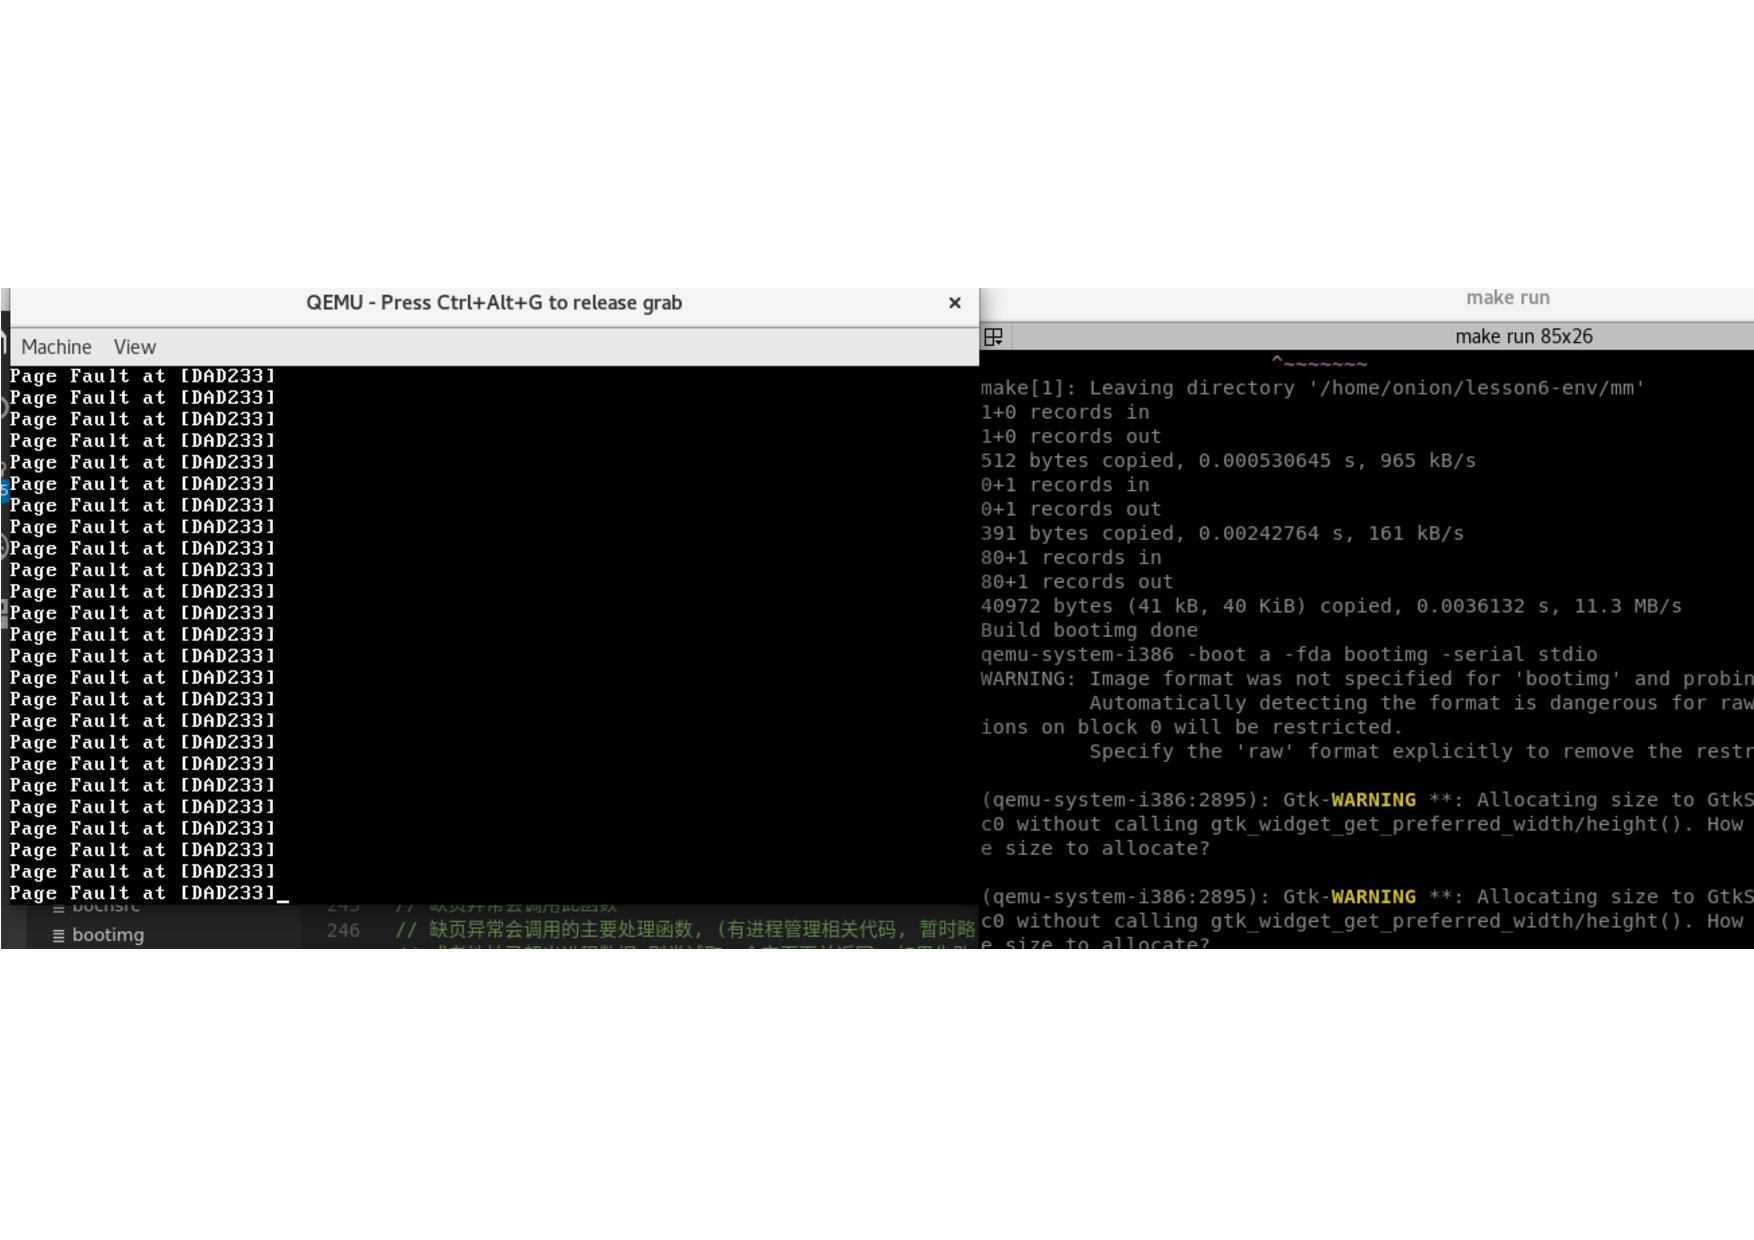
\includegraphics[width=\textwidth]{img/缺页异常时的无限中断.pdf}
    \caption{缺页异常时的无限中断}
    \label{fig:缺页异常时的无限中断}
\end{figure}

\begin{mdframed}[hidealllines=true,backgroundcolor=gray!20]
\textbf{练习 }进入实验环境目录下 mm/memory.c 文件,找到 do\_no\_page,do\_wp\_page,un\_wp\_page 函数,其中,do\_no\_page 为缺页处理函数,该函数在发生缺页异常时会调用get\_free\_page 函数申请一页物理内存,接下来将该 page 映射到指定的线性地址 address 处,若操作成功则返回,否则释放内存页,并调用 oom 函数报错。(此处暂不考虑进程管理以及页面共享,故代码与 Linux 0.11 内核有一定区别)

请尝试完成 do\_no\_page 函数,之后运行 NEUOS,便可以看到缺页异常提示以及申请的新的页信息,如图 \ref{fig:内存函数测试} 所示。
\end{mdframed}

\begin{figure}[htbp]
    \centering
    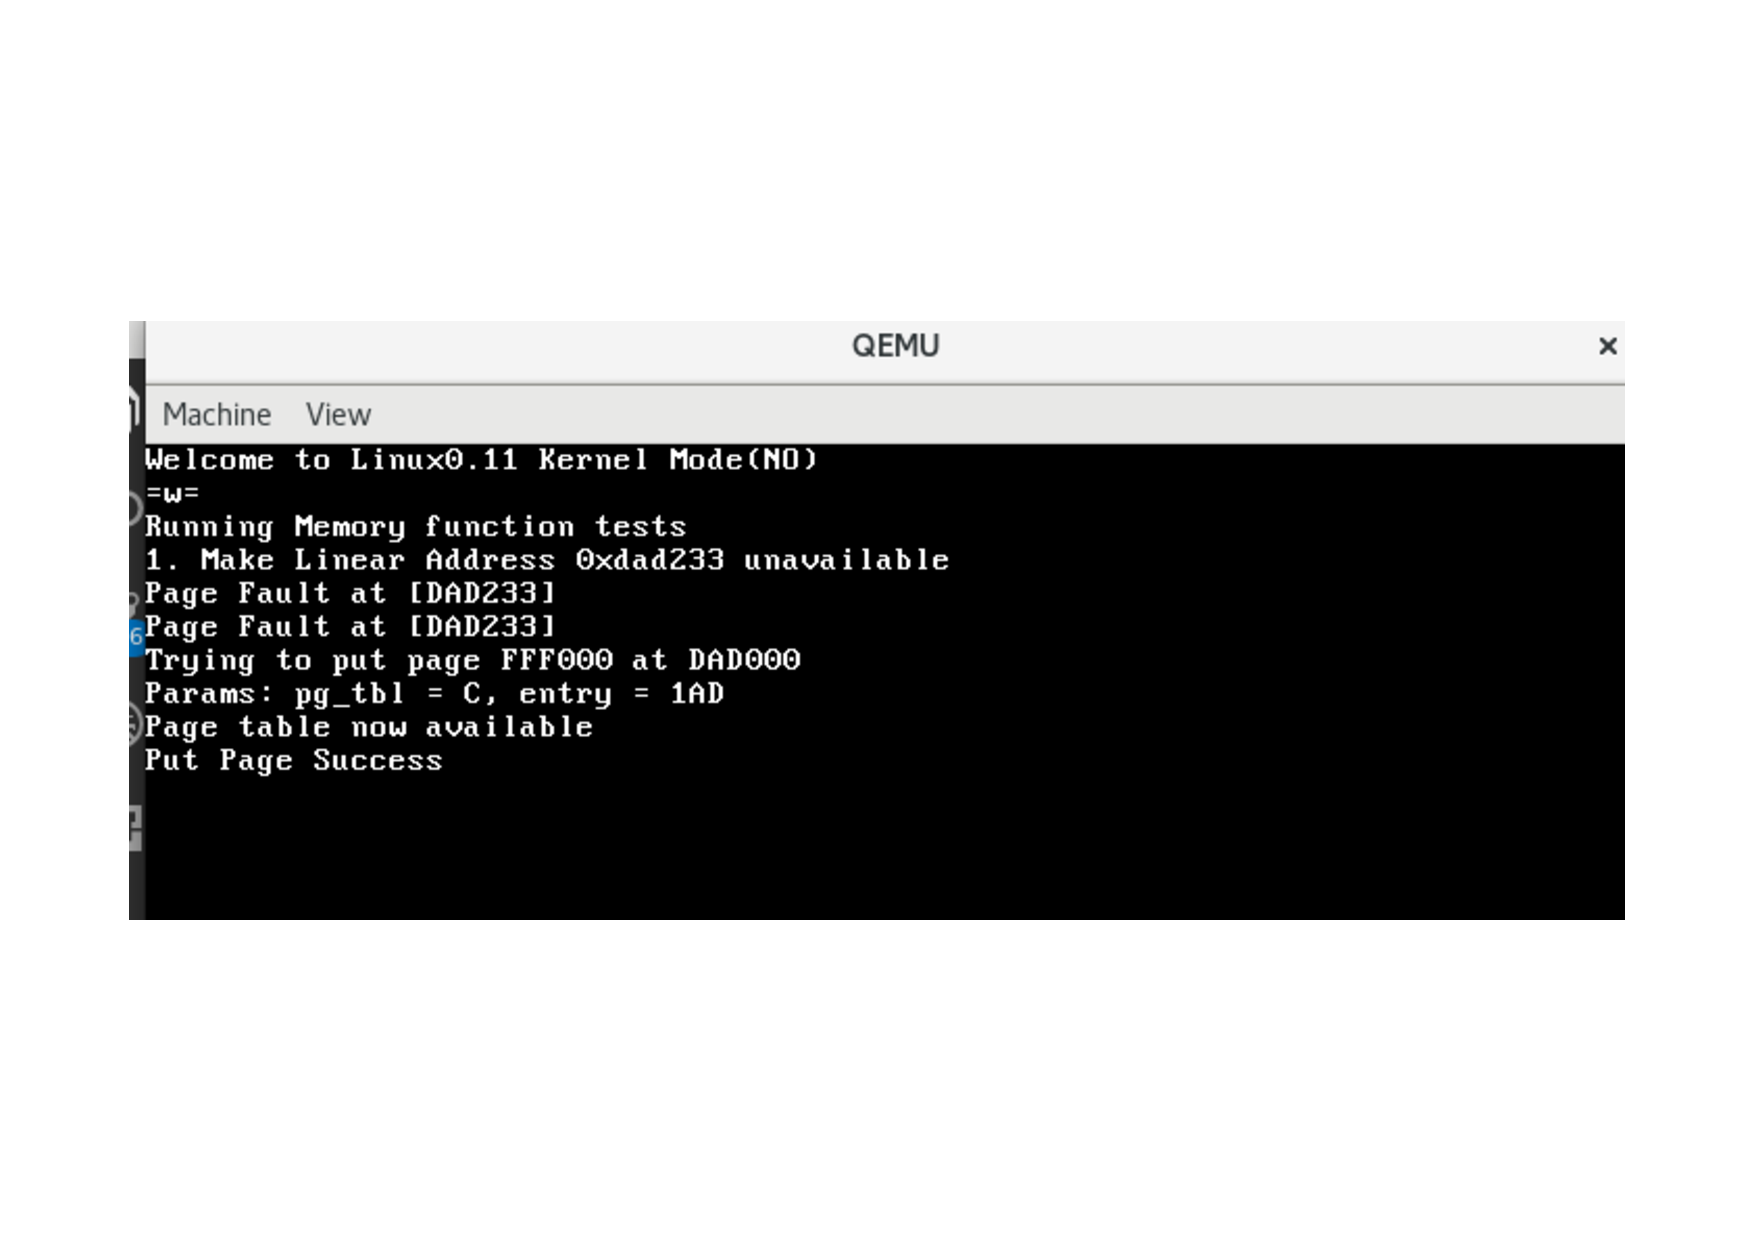
\includegraphics[width=\textwidth]{img/内存函数测试.pdf}
    \caption{内存函数测试}
    \label{fig:内存函数测试}
\end{figure}

\begin{mdframed}[hidealllines=true,backgroundcolor=gray!20]
\textbf{练习 }读懂 exp5/mm/memory.c 中的 do\_wp\_page 函数调用 un\_wp\_page 时传递的 table\_entry 表达式,并描述出具体含义。其中,table\_entry 是 un\_wp\_page 函数所需的参数。
\end{mdframed}

\begin{mdframed}[hidealllines=true,backgroundcolor=gray!20]
\textbf{练习 }根据实验四所学串口知识及相关代码,在 exp5/kernel/serial.c 实现空缺的函数。在 exp5/include/linux/kernel.h 中这些函数已有声明,Makefile 中的 OBJS 也已补充。

将 exp5/mm/memory.c 源文件中 do\_no\_page 函数中的 printk(“Page Fault at... 修改为 s\_printk(“Page Fault at…

编译后使用 QEMU 运行 NEUOS 后即可在终端中看到串口输出的缺页异常信息,如图 \ref{fig:缺页异常信息} 所示。
\end{mdframed}

\begin{figure}[htbp]
    \centering
    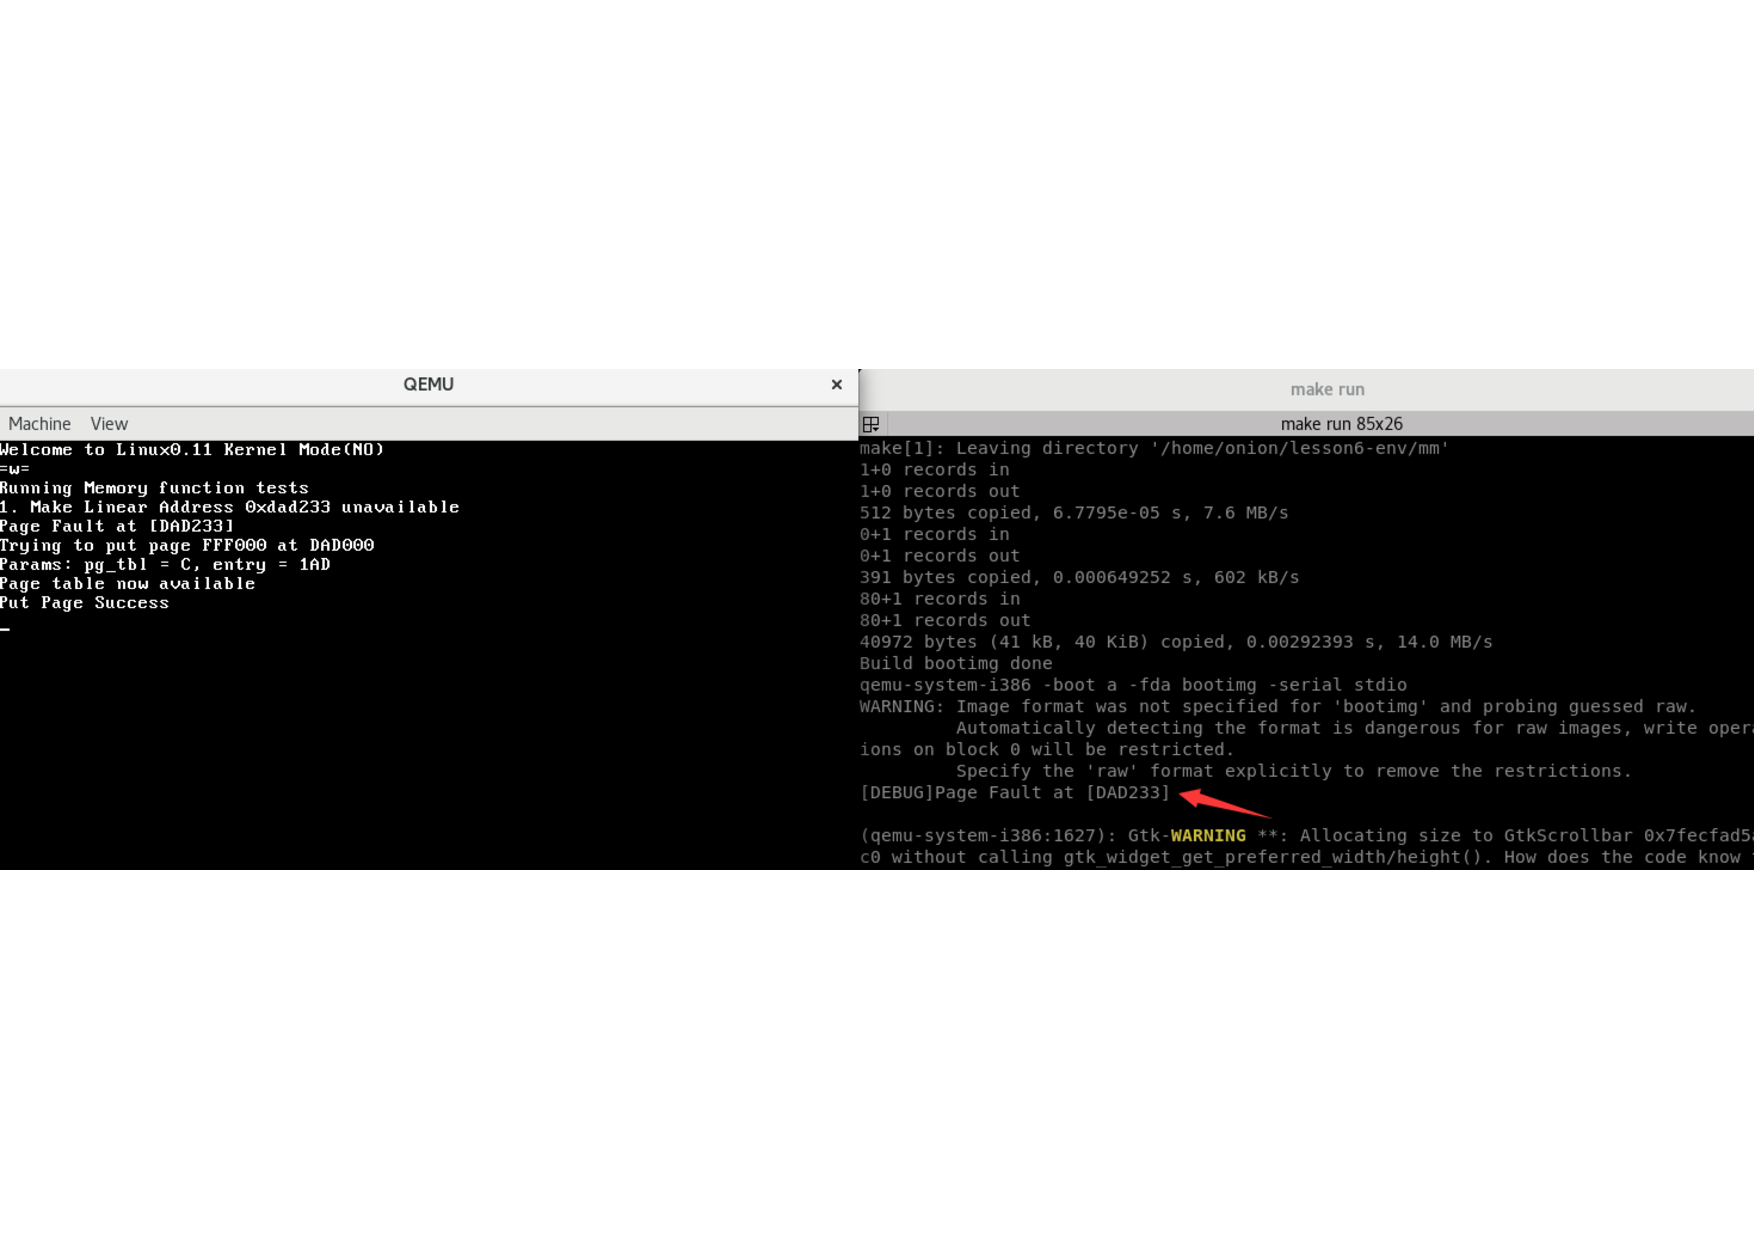
\includegraphics[width=\textwidth]{img/缺页异常信息.pdf}
    \caption{缺页异常信息}
    \label{fig:缺页异常信息}
\end{figure}

接下来,在 QEMU 的 log 中找到中断发生时的寄存器信息。

提示:qemu-system-i386 -d 命令用于输出 log 信息,要输出中断的 log 信息,尝试使用 qemu-system-i386 -d help 命令找到输出中断信息的命令。然后,补充 exp5/Makefile 中的 run 命令,使用 make run 运行 NEUOS,如图 \ref{fig:QEMU中断日志} 所示。请描述你是如何使用 QEMU 查看中断信息的,并展示运行截图。

\begin{figure}[htbp]
    \centering
    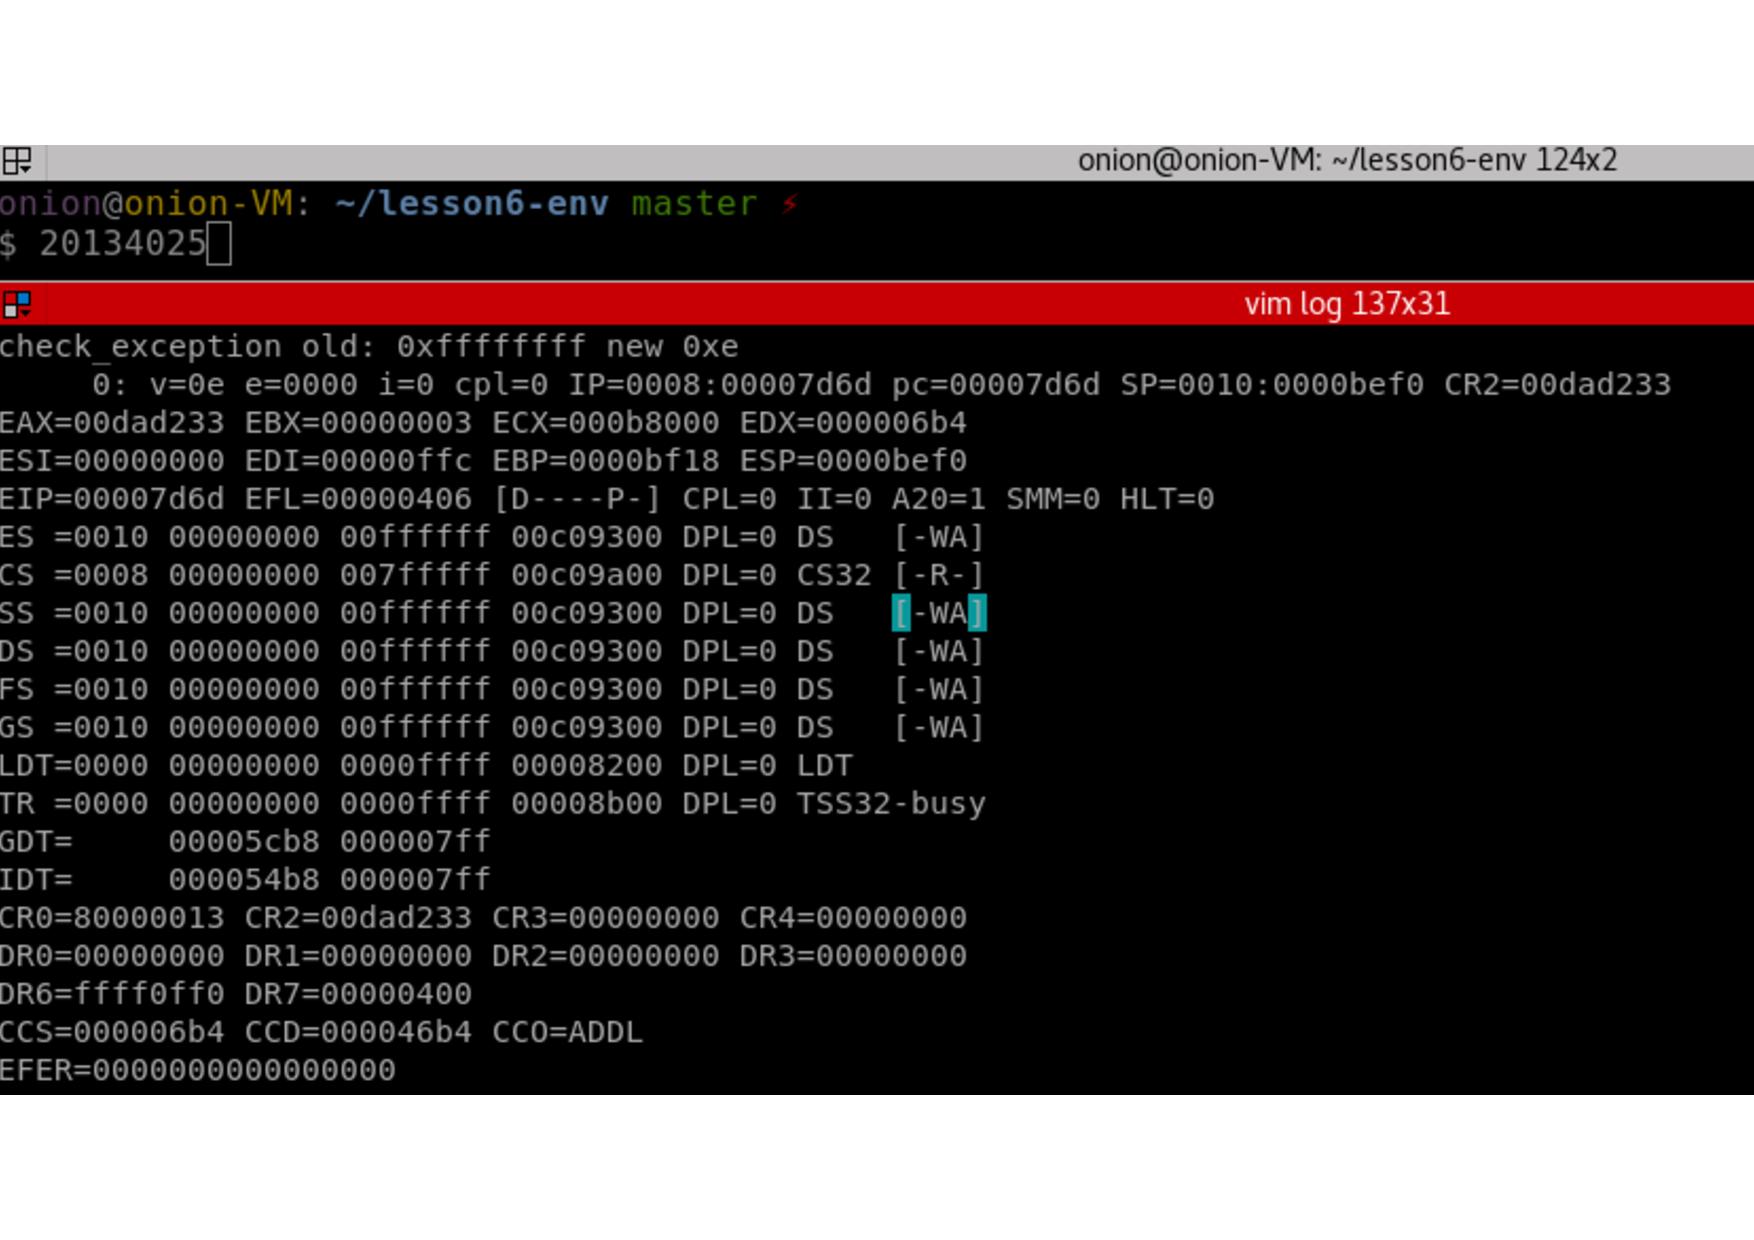
\includegraphics[width=\textwidth]{img/QEMU中断日志.pdf}
    \caption{QEMU 中断日志}
    \label{fig:QEMU中断日志}
\end{figure}

